\section{Appendix: Simple 3-connected monochromatic blinks up to 16 edges}
\label{chap:catalolgue3con}

We here present all simple 3-connected green blinks with
$\leq 16$ edges divided in 381 HGnQI classes. The quantum
invariant was calculated up to level $r=8$ for each of
these blinks. There are left 11 uncertainties: 14.24t,
15.16t, 15.19t, 15.22t, 16.42t, 16.56t, 16.141t, 16.142t,
16.149t, 16.233t. Except for these classes the other 370
consisted of only one blink (or the two orientations of
the same space). This fact suggests that if $A$ and $B$
are two different simple 3-connected monochromatic blinks,
that do not form a trivial pair (trivially induce the
same space), then they probably induce different spaces.
Are the 11 uncertainties examples of non-trivial pairs?

\begin{center}
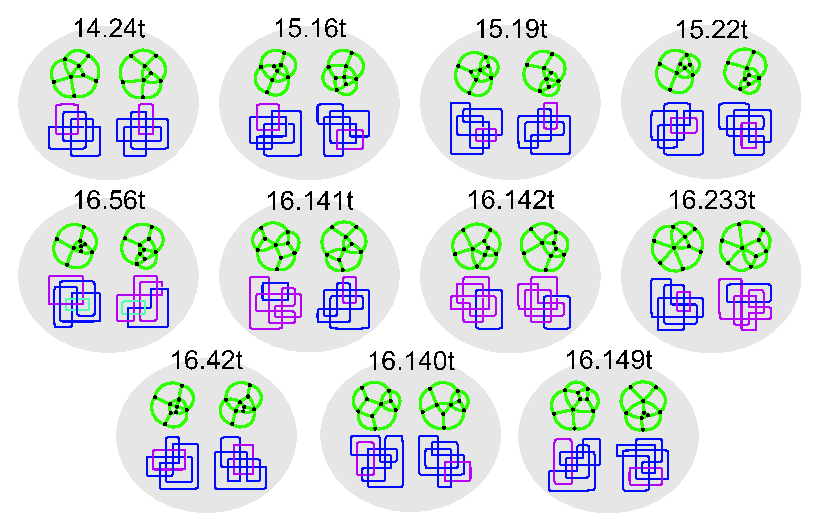
\includegraphics{A.figs/doubts3connectedisolated.eps}
\end{center}

\setlength{\topmargin}{-1.2cm}
%\setlength{\textwidth}{\paperwidth-2in}
%\setlength{\headheight}{1cm}
%\setlength{\headsep}{-3cm}
%\setlength{\footskip}{0.1cm}
%\setlength{\textheight}{\paperheight-\headheight-\headsep-\footskip-2in}
%\setlength{\oddsidemargin}{0mm}
%\setlength{\evensidemargin}{0mm}
%\setlength{\marginparwidth}{0mm}
%\setlength{\marginparsep}{0mm}
%\setlength{\textwidth}{\paperwidth-2in}

\begin{center}
 \includegraphics[height=23.5cm]{E.figsbw2/con3catalog001_bw.pdf} \eject
 \includegraphics[height=23.5cm]{E.figsbw2/con3catalog002_bw.pdf} \eject
 \includegraphics[height=23.5cm]{E.figsbw2/con3catalog003_bw.pdf} \eject
 \includegraphics[height=23.5cm]{E.figsbw2/con3catalog004_bw.pdf} \eject 
 \includegraphics[height=23.5cm]{E.figsbw2/con3catalog005_bw.pdf} \eject
 \includegraphics[height=23.5cm]{E.figsbw2/con3catalog006_bw.pdf} \eject
 \includegraphics[height=23.5cm]{E.figsbw2/con3catalog007_bw.pdf} \eject
 \includegraphics[height=23.5cm]{E.figsbw2/con3catalog008_bw.pdf} \eject 
 \includegraphics[height=23.5cm]{E.figsbw2/con3catalog009_bw.pdf} \eject
 \includegraphics[height=23.5cm]{E.figsbw2/con3catalog010_bw.pdf} \eject
 \includegraphics[height=23.5cm]{E.figsbw2/con3catalog011_bw.pdf} \eject
 \includegraphics[height=23.5cm]{E.figsbw2/con3catalog012_bw.pdf} \eject 
 \includegraphics[height=23.5cm]{E.figsbw2/con3catalog013_bw.pdf} \eject
 \includegraphics[height=23.5cm]{E.figsbw2/con3catalog014_bw.pdf} \eject
 \includegraphics[height=23.5cm]{E.figsbw2/con3catalog015_bw.pdf} \eject
 \includegraphics[height=23.5cm]{E.figsbw2/con3catalog016_bw.pdf} \eject  
 \includegraphics[height=23.5cm]{E.figsbw2/con3catalog017_bw.pdf} \eject
 \includegraphics[height=23.5cm]{E.figsbw2/con3catalog018_bw.pdf} \eject
 \includegraphics[height=23.5cm]{E.figsbw2/con3catalog019_bw.pdf} \eject
 \includegraphics[height=23.5cm]{E.figsbw2/con3catalog020_bw.pdf} \eject 
 \includegraphics[height=23.5cm]{E.figsbw2/con3catalog021_bw.pdf} \eject
 \includegraphics[height=23.5cm]{E.figsbw2/con3catalog022_bw.pdf} \eject
 \includegraphics[height=23.5cm]{E.figsbw2/con3catalog023_bw.pdf} \eject
 \includegraphics[height=23.5cm]{E.figsbw2/con3catalog024_bw.pdf} \eject 
 \includegraphics[height=23.5cm]{E.figsbw2/con3catalog025_bw.pdf} \eject
 \includegraphics[height=23.5cm]{E.figsbw2/con3catalog026_bw.pdf} \eject
 \includegraphics[height=23.5cm]{E.figsbw2/con3catalog027_bw.pdf} \eject
 \includegraphics[height=23.5cm]{E.figsbw2/con3catalog028_bw.pdf} \eject 
 \includegraphics[height=23.5cm]{E.figsbw2/con3catalog029_bw.pdf} \eject
 \includegraphics[height=23.5cm]{E.figsbw2/con3catalog030_bw.pdf} \eject
 \includegraphics[height=23.5cm]{E.figsbw2/con3catalog031_bw.pdf} \eject
 \includegraphics[height=23.5cm]{E.figsbw2/con3catalog032_bw.pdf} \eject  
 \includegraphics[height=23.5cm]{E.figsbw2/con3catalog033_bw.pdf} \eject
 \includegraphics[height=23.5cm]{E.figsbw2/con3catalog034_bw.pdf} \eject  
 \includegraphics[height=23.5cm]{E.figsbw2/con3catalog035_bw.pdf} \eject
 \includegraphics[height=23.5cm]{E.figsbw2/con3catalog036_bw.pdf} \eject  
 \includegraphics[height=23.5cm]{E.figsbw2/con3catalog037_bw.pdf} \eject
 \includegraphics[height=23.5cm]{E.figsbw2/con3catalog038_bw.pdf} \eject  
 \includegraphics[height=23.5cm]{E.figsbw2/con3catalog039_bw.pdf} \eject
\end{center}
 
% \newcount\ii \newcount\jj   % declare integer variable
% \def\producePagesThree#1#2{
% \ii=#1                      % initialize ii
% \jj=#2                      % initialize jj
% \advance\jj by 1            % increment jj
% \loop   % loop
%    \ifnum\ii<\jj
% {
%    %\vspace{-1cm}
%    %\thispagestyle{empty}
%    % \setlength{\hoffset}{0cm}
%    % \setlength{\textwidth}{\paperwidth-2cm}
%    \hspace{-1.8cm}
%    \enlargethispage{5cm}
%    {\centering
%    \includegraphics[height=23.5cm]{E.figsbw2/con3catalog\ifnum\ii<100 0\fi\ifnum\ii<10 0\fi\number\ii.eps}
%    }
%    \newpage}
%       \advance\ii by 1
%    \repeat
% }


%\newlength{\topmarginOne}
%\setlength{\topmarginOne}{\topmargin}
%\setlength{\topmargin}{\topmarginOne}
